% Imporditud: tools/import_eksperimendid.py
% Allikas: Eesti füüsikaolümpiaadi eksperimendi ülesannete
%   kogu (Rael Kalda, 2023), ülesanne Ü44, lahendus L44.
\setAuthor{EFO žürii}
\setRound{lõppvoor}
\setYear{2002}
\setNumber{P E1}
\setDifficulty{2}
\setTopic{vedelike mehaanika}
\setVahendid{anum veega, keha, niit, dünamomeeter, mõõtejoonlaud}
\setPunktid{10}
\setAllikas{Eksperimendi kogu Ü44, lahendus lk 53}
\setLahendusseis{toores}

\prob{Keha vees}
Keha asub vees. Määrake minimaalne töö, mis tuleb teha keha tõstmiseks põhjast pinnale (vt. joon.). Hinnake tulemuse täpsust.
\begin{center}
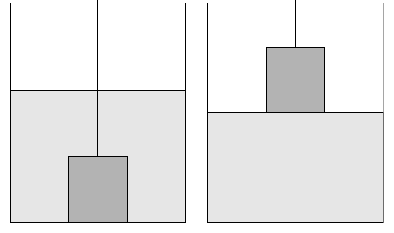
\includegraphics[width=0.30\linewidth]{2002-v3g-pe1-yl.png}
\end{center}

\hint

\solu
Tähistused: $h_1$ on kõrgus, milleni tuleb keha tõs- F $A_1$ ta, et keha ülemine tahk oleks veepinna nivool. $h_2$ $F_2$ on kõrgus, milleni tuleb keha tõsta, et keha alu-

mine tahk oleks veepinna nivool. $F_1$ on jõud keha $F_1$ tõstmiseks, kui keha on täielikult sukeldatud vet-

te. $F_2$ on jõud keha hoidmiseks, kui keha on täie- $A_2$ h likult veest väljas. Mõõtmistulemuste põhjal koos-

tatud graafik omab joonisel toodud kuju. Graafiku-

joone alune pindala teljestikus antud suurustes on $h_1$ $h_2$

minimaalne töö keha tõstmiseks. Kogu töö on ots-

tarbekas leida kahe osatöö summana: A = $A_1$ +$A_2$,

kus $A_1$ = F1h ja

$A_2$ = ($F_2$ $-$ $F_1$)($h_2$ $-$ $h_1$ ) 2 .

Tulemuse täpsuse hinnang on kvalitatiivne näidates ära peamised mõõtmise ebatäpsuse allikad.
\probend
